\documentclass[12pt, a4paper]{article}

\usepackage[polish]{babel}
\usepackage[utf8]{inputenc}
\usepackage{polski}	
\usepackage{algpseudocode,algorithm,algorithmicx}
\frenchspacing	
\usepackage{graphics}
\usepackage{graphicx}
	
\title{\textbf{Obliczenia naukowe\\Lista 4}}
\author{Mateusz Kościelniak 244973\\}
\date{Grudzień 2019}

\begin{document}

\maketitle

\newpage

\section{Zadanie 1}
\subsection{Opis problemu}
Implementacja funkcji obliczającej iloraz różnicowy zadanych węzłow oraz odpowiadających im wartości, bez użycia tablicy dwuwymiarowej. 
\subsection{Rozwiązanie}
Iloraz różnicowy k-tego rzędu można obliczyć za pomocą wzoru rekurencyjnego:

$$
y = \left\{ \begin{array}{ll}
f[x_i]=f(x_i) & \textrm{dla k = 0}\\
f[x_i,x_j] = \frac{f(x_j) - f(x_i)}{x_j - x_i} & \textrm{dla k = 1}\\
f[x_i,x_{i+1}, \ldots, x_{i+k}] = \frac{f[x_{i+1},x_{i+2}, \ldots, x_{i+k}] - f[x_{i}, x_{i+1}, \ldots, x_{i+k-1}]}{x_k - x_i} & \textrm{dla k > 1}
\end{array} \right.
$$

Patrząc na to równanie możemy stwierdzić, że kolejne ilorazy różnicowe zależą od poprzednich, a  tą zależność możemy zobrazować za pomocą tablicy, oznaczmy  
$c_{ij} = f[x_i, \ldots, x_{i+j}]$, teraz mamy:

\begin{table}[h]
        \centering
        \footnotesize
        \renewcommand{\arraystretch}{1.5}
\begin{tabular}{l} 
$c_{0,0} $ \quad $c_{0,1}$ \quad $c_{0,2}$ \quad \ldots \quad $c_{0,k-1}$ \quad $c_{0,k}$ \\
$c_{1,0} $ \quad $c_{1,1}$ \quad $c_{1,2}$ \quad \ldots \quad $c_{1,k-1}$ \\
\ldots \quad \ldots \quad \ldots \\
$c_{k-1,0}$ \quad $c_{k-1,1}$ \\
$c_{k,0}$ \\
\end{tabular}
\caption{Ilorazy różnicowe.}
\end{table}

Najwygodniejszym lecz nie najoptymalniejszym sposobem byłoby użycie tablicy dwuwymiarowej, lecz kierując się poleceniem użyłem tablicy jednowymiarowej. Wartośc współczynników $c_{i,j}$ z powyższej tablicy, można wyrazić wzorem $c_{ij} = \frac{c_{i+1,j-1} - c_{i,j-1}}{x_{i+j} - x_{i}}$, na początku tablica ilorazów różnicowych fx przechowuje wartości $fx[i]=c_{i,0}=f(x_i)$, natomiast kolejne wartości to odpowiednio $c_{i-1, 1}, \ldots, c_{1,i-1}, c_{0i}$. W każdej iteracji algorytmu otrzymywane są kolejne kolumny w tablicy pierwszej niezbędne do wyliczenia kolejnych ilorazów różnicowych.

\newpage

\section{Zadanie 2}
\subsection{Opis problemu}
Implementacja funkcji obliczającej wartość wielomianu interpolacyjnego stopnia $n$ w postaci Newtona $N_n(x)$ w punkcie $x=t$ za pomocą uogólnionego algorytmu Hornera. Czas algorytmu powinien być $O(n)$.
 
\subsection{Rozwiązanie}
Algorytm Hornera dla tego przypadku wygląda następująco\\\\
$w_{n}(x) = f[x_{0}, x_{1}, \ldots, x_{n}]$ \\
$w_{k}(x) = f[x_{0}, x_{1}, \ldots, x_{k}] + (x - x_{k})w_{k+1}(x)$, gdzie $(k = n - 1, \ldots, 0)$ \\
$N_{n}(x) = w_{0}(x)$. \\\\

Na podstawie powyższych wzorów można napisać algorytm wyznaczający wartość wielomianu w czasie $O(n)$, gdzie głowne obliczenia są wykonywane w pętli:

\begin{algorithm}
    \begin{algorithmic}[1]
            \For{$i \gets n - 1$ \textbf{downto} $1$}
                \State $n_{t} \gets f_{x}[i] + (t - x[i]) \cdot n_{t}$
            \EndFor
    \end{algorithmic}
\end{algorithm} 

\textbf{Opis parametrów:} \\
\texttt{x} - wektor długości $n + 1$ zawierający węzły $x_{0}, \ldots, x_{n}$, \\
\texttt{$f_x$} - wektor długości $n + 1$ zawierający obliczone ilorazy różnicowe \\
\texttt{t} - punkt, w którym należy obliczyć wartość wielomianu\\
\texttt{$n_t$} - wartość wielomianu w punkcie $t$\\\\


\newpage

\section{Zadanie 3}
\subsection{Opis problemu}
Znając współczynniki wielomianu interpolacyjnego w postaci Newtona oraz węzły należało zaimplementować funkcję obliczającą w czasie $O(n^2)$ współczynniki jego postaci naturalnej.

\subsection{Rozwiązanie}
W celu znalezienia współczynników wielomianu wykorzystałem uogólniony algorytm Hornera z poprzedniego zadania. Wykorzystałem fakt, że w wielomianie interpolacyjnym n-tego stopnia, współczynnik $a_n$ przy najwyższej potędze x jest równy $c_n$, a $w_n$ z uogólnionego algorytmu hornera jest równy $a_n$. Teraz w pętli wyliczamy kolejne wartości częsciowe dla wielomianu interpolacyjnego, z tą różnicą, że podczas każdej iteracji chcemy uzyskać współczynniki dla postaci naturalnej wielomianu interpolacyjnego.\\

\begin{algorithm}
    \begin{algorithmic}[1]
        \Function{naturalna}{$x, f_{x}$}
            \State $n \gets$ \Call{length}{$x$}
            \State $a[n] \gets f_x[n]$

            \For{$i \gets n - 1$ \textbf{downto} $1$}
                \State $a[i] = f_{x}[i] - a[i+1] \cdot x[i]$
                \For{$j \gets i + 1 $ \textbf{to} $n - 1$}
                    \State $a[j] \gets a[j] - a[j + 1] \cdot x[i]$
                \EndFor
            \EndFor
            \State \Return $a$
        \EndFunction
    \end{algorithmic}
\end{algorithm} 

\textbf{Opis parametrów:} \\
\texttt{x} - wektor długości $n + 1$ zawierający węzły $x_{0}, \ldots, x_{n}$, \\
\texttt{fx} - wektor długości $n + 1$ zawierający obliczone ilorazy różnicowe \\
\texttt{a} - wektor długości $n + 1$ zawierający obliczone współczynniki postaci naturalnej.\\\\

Widzimy, że pętla zewnętrzna jak  i wewnętrzna wykonają się co najwyżej n-1 razy 
co daje złożoność przedstawionego powyżej algorytmu rzędu $O(n^2)$.

\section{Zadanie 4}
\subsection{Opis problemu}
Implementacja algorytmu interpolującego funkcję $f(x)$ w przedziale $[a, b]$ za pomocą wielomianu interpolacyjnego stopnia n w postaci Newtona. Następnie narysowanie wielomianu interpolacyjnego oraz interpolowanej funkcji. Dodatkowo w interpolacji należało użyć węzłów równoodległych.

\subsection{Rozwiązanie}
Na początku wyznaczyłem węzły interpolacji $(x_1,\dots,x_{n+1})$, które są równoległe, rozmieszczone w odległości $\frac{b-a}{n}$ w przedziale $[a, b]$ oraz wartości funkcji w stworzonych węzłach. Następnie przy pomocy wcześniej zaimplementowanej funkcji \texttt{ilorazyRoznicowe} obliczyłem ilorazy różnicowe dla stworzonych wcześniej węzłów, następnie za pomocą funkcji \texttt{warNewton} obliczylem wartości wielomianu w kolejnych węzłach. Po wykonaniu tych działań miałem już dostateczne dane do narysowania funckji $f$ oraz jej wielomianu interpolacyjnego.
										
\section{Zadanie 5}
\subsection{Opis problemu}
Testowanie funkcji \texttt{rysujNfx} na przykładach:
\begin{itemize}
    \item[(a)] $e^{x}$, $[0, 1]$, $n = 5, 10, 15$,
    \item[(b)] $x^{2} \sin x$, $[-1, 1]$, $n = 5, 10, 15$.
\end{itemize}

\subsection{Rozwiązanie}
Dla zadanych danych wywołano funkcję \texttt{rysujNfx} zaimplementowaną w zadaniu 4.

\newpage

\subsection{Wyniki}

\begin{figure}[h]
    \centering
    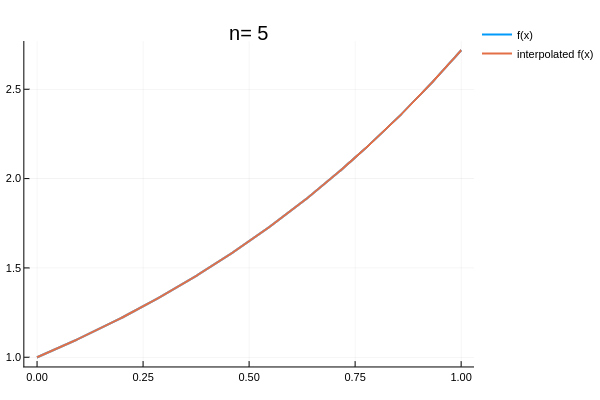
\includegraphics[scale=0.35]{../plots/ex5/1.png}
    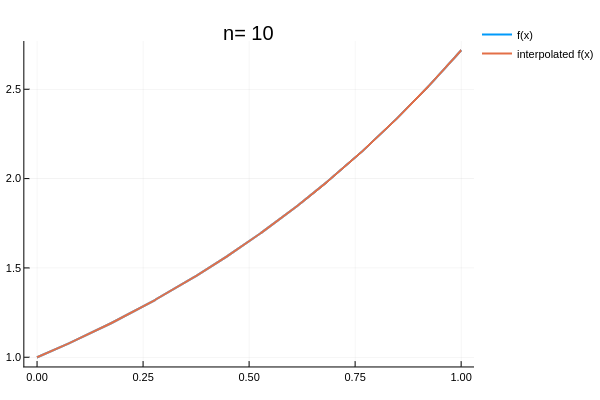
\includegraphics[scale=0.35]{../plots/ex5/4.png}
    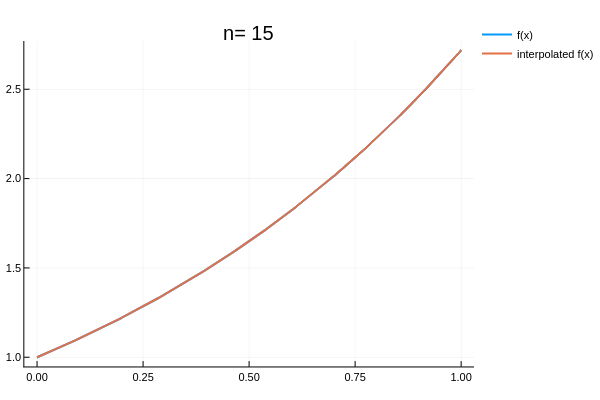
\includegraphics[scale=0.35]{../plots/ex5/3.png}    
    \caption{Wykresy dla funkcji $e^x$}
\end{figure}

\newpage

\begin{figure}[h]
    \centering
    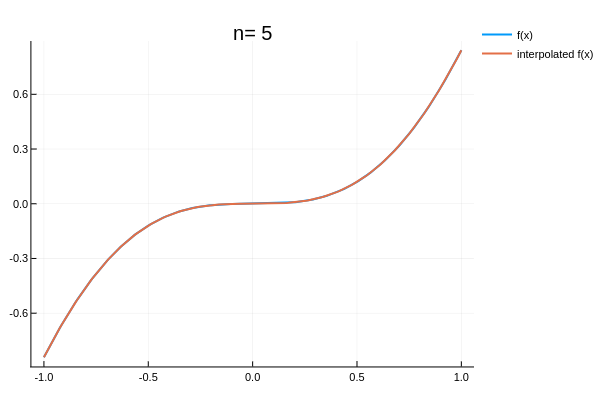
\includegraphics[scale=0.35]{../plots/ex5/2.png}
    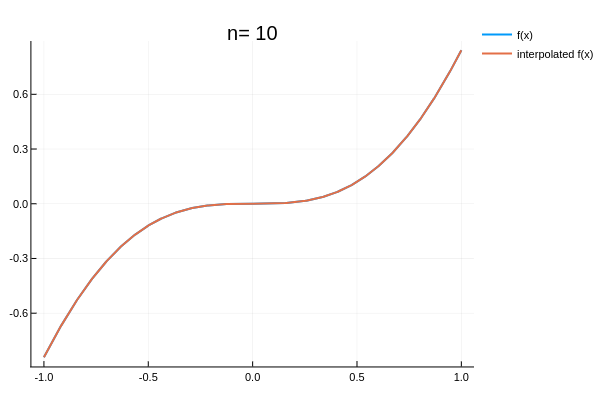
\includegraphics[scale=0.35]{../plots/ex5/5.png}
    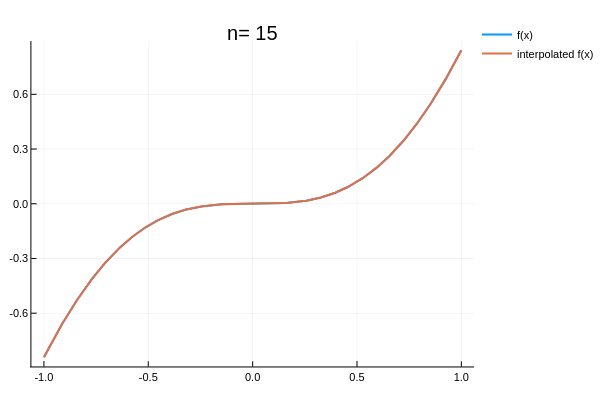
\includegraphics[scale=0.35]{../plots/ex5/6.png}    
    \caption{Wykresy dla funkcji $x^2*sin(x)$}
\end{figure}

\newpage

\subsection{Wnioski}
Dla funkcji $e^x$ jak i $x^2\sin{x}$ na zadanych przedziałach wielomiany interpolacyjne są bardzo bliskie interpolowanym funkcją, na powyższych  wykresach róznice są niewidoczne. Widać zatem że w tym przypadku zastosowanie równoodległych węzłów interpolacji dało bardzo dobre przybliżenia interpolowanych funkcji.



\section{Zadanie 6}
\subsection{Opis problemu}
Testowanie funkcji \texttt{rysujNfx} na przykładach:
\begin{itemize}
    \item[(a)] $|x|$, $[0, 1]$, $n = 5, 10, 15$,
    \item[(b)] $\frac{1}{1 + x^{2}}$, $[-5, 5]$, $n = 5, 10, 15$ (zjawisko Runge'go).
\end{itemize}


\subsection{Rozwiązanie}
Dla zadanych danych wywołano funkcję \texttt{rysujNfx} zaimplementowaną w zadaniu 4.

\newpage

\subsection{Wyniki}

\begin{figure}[h]
    \centering
    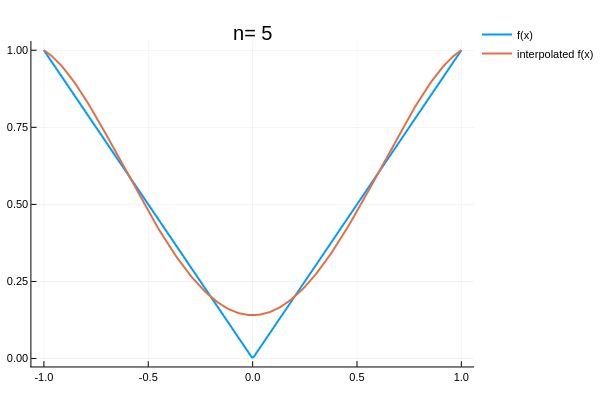
\includegraphics[scale=0.35]{../plots/ex6/1.png}
    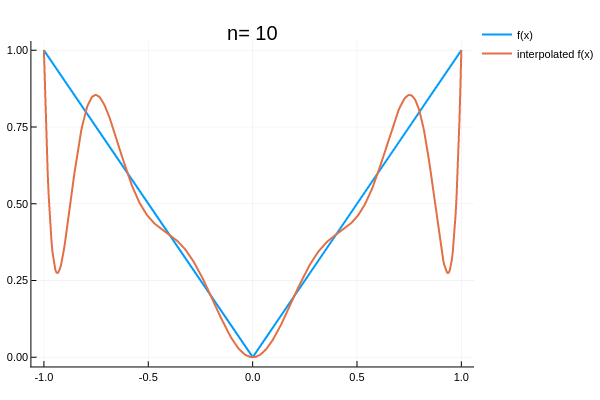
\includegraphics[scale=0.35]{../plots/ex6/2.png}
    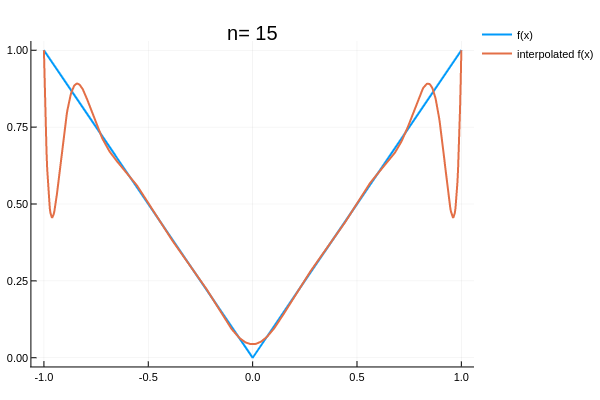
\includegraphics[scale=0.35]{../plots/ex6/3.png}    
    \caption{Wykresy dla funkcji $|x|$}
\end{figure}

\newpage

\begin{figure}[h]
    \centering
    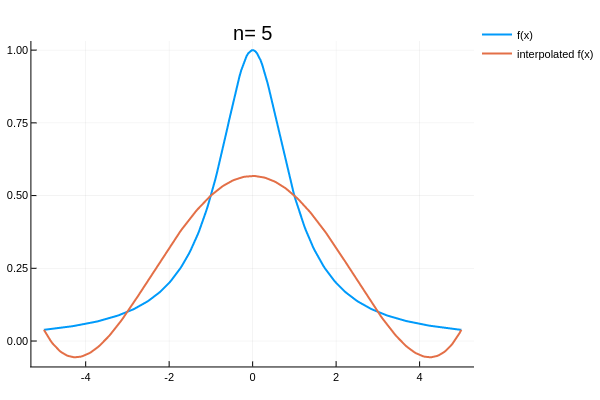
\includegraphics[scale=0.35]{../plots/ex6/4.png}
    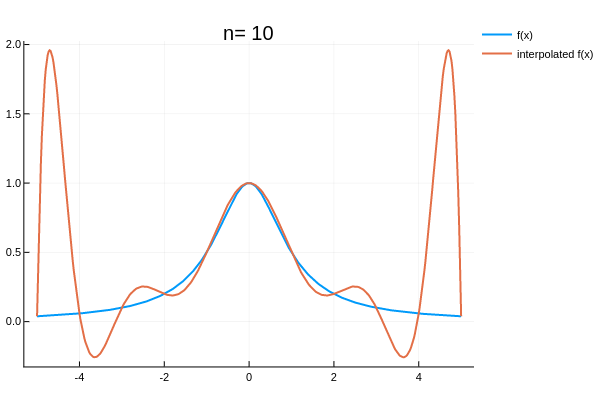
\includegraphics[scale=0.35]{../plots/ex6/6.png}
    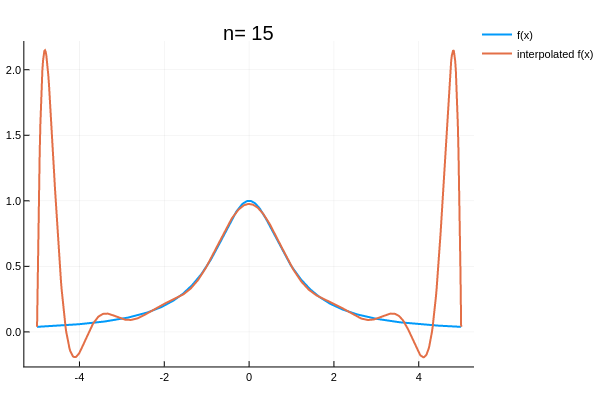
\includegraphics[scale=0.35]{../plots/ex6/5.png}    
    \caption{Wykresy dla funkcji $\frac{1}{1+x^2}$}
\end{figure}

\subsection{Wnioski}
W przypadku funkcji $f(x) = |x|$ zjawisko rozbieżności wynika z tego, że funkcja ta nie jest różniczkowalna.
Dla funkcji $f(x) = \frac{1}{1+x^{2}}$ mamy do czynienia z efektem Runge'go. 
Polega ono pogorszeniu się jakości interpolacji wielomianowej, mimo zwiększenia liczby jej węzłów, co jest szczególnie widoczne na końcach przedziałów jest to typowe zjawisko dla interpolacji za pomocą wielomianów wysokich stopni przy stałych odległościach węzłów. W celu przeciwdziałania temu efektowi stosuje się interpolację, w której węzły są gęściej rozmieszczone na krańcach przedziału, na którym funkcja jest interpolowana. Można zastosować wtedy wielomiany Czebyszewa $n$-tego stopnia, których miejsca zerowe stają się węzłami. Wiemy bowiem, że dla takich wielomianów ich miejsca zerowe są gęściej rozmieszczone na zadanym przedziale. 
Warto również wspomnieć, że zjawisko Runge'go występuje również, gdy interpolowana funkcja jest nieciągła albo odbiega znacząco od funkcji gładkiej.

\end{document}
